% !TeX root = ../ecuaciones-diferenciales.tex

\chapter{Ecuaciones de orden superior}
\section{Ecuaciones lineales de orden II}

\begin{thm}[Existencia y unicidad para ecuaciones lineales de orden II]\label{thm:exist-unic-ii}
    Sean: \\$(\mathcal{EC}) \equiv \mbf{x}'' + p(t)\mbf{x}' + q(t) \mbf{x} = r(t)$ con $p, q, r: [a, b] \subset \R \to \R$ continuas y $t_0 \in [a, b]$, $x_0,\ x_1 \in R$ entonces existe una solución y es única al PVI:
    $$
        \begin{cases}
            \mbf{x}'' + p(t)\mbf{x}' + q(t)\mbf{x} = r(t),\ \forall t \in [a, b].\\
            x(t_0) = x_0\\
            x'(t_0) = x_1\\
        \end{cases}
    $$
\end{thm}
La demostración de nuevo se deja para el caso general.\\\\
Vamos a enunciar ciertas \textbf{propiedades}.
\begin{enumerate} \label{properties:ecua-lin-ii}
    \item Es lineal, el conjunto de soluciones es un espacio vectorial.
    $$
        \text{Sean } \mbf{x}_1, \mbf{x}_2 \text{ soluciones de la homogénea, } \alpha_1, \alpha_2 \in \R \implies \alpha_1 x_1(t) + \alpha_2 x_2(t) \text{ es solución de la homogénea.}
    $$
    \item Ese espacio vectorial tiene dimensión 2.
\end{enumerate}
\begin{proof} (\textit{de las propiedades})\\
    \begin{enumerate}
        \item Se demuestra como en el ejemplo.
        \item Sea $x_1$ la solución del PVI:
        $$
        \begin{cases}
            \mbf{x}'' + p(t) \mbf{x}' + q(t) \mbf{x} = 0\\
            x(a) = 1\\
            x'(a) = 0
        \end{cases}
        $$
        y sea $x_2$ la solución del PVI:
        $$
        \begin{cases}
            \mbf{x}'' + p(t) \mbf{x}' + q(t) \mbf{x} = 0\\
            x(a) = 0\\
            x'(a) = 1
        \end{cases}
        $$
        Por existencia y unicidad, $\mbf{x}_1, \mbf{x}_2$ existen en $[a,b]$. Además, ninguna es un múltiplo de la otra, es decir, son linealmente independientes pues:
        \begin{itemize}
            \item Cualquier $\mbf{x} = \alpha \mbf{x}_1$ cumple $x'(a) = 0$ pero $x_2'(a) \neq 0$.
            \item Cualquier $\mbf{x} = \beta \mbf{x}_2$ cumple $x(a) = 0$ pero $x_1(a) \neq 0$.
        \end{itemize}
        Por tanto, la dimensión del espacio de soluciones es al menos 2. Para ver que es justo dos se sigue:\\\\
        Dada cualquier solución x(t) de la ecuación
        $$
            x(t) = x(a) \cdot x_1(t) + x'(a) \cdot x_2(t)
        $$ %%TODO: Clarificar.
        por unicidad, el término de la derecha es solución con:
        $$
            \begin{cases}
                \text{ valor en a igual a $x(a)$}\\
                \text{ derivada en a igual a $x'(a)$}
            \end{cases}
        $$
    \end{enumerate}
\end{proof}

\begin{obs}
    Como vimos en el ejemplo \ref{eg:muelle}, para resolver $\mbf{x}'' + p(t) \mbf{x}' + q(t) \mbf{x} = 0$ basta encontrar dos soluciones linealmente independientes.
\end{obs}

\begin{eg}[Ecuaciones de orden II como sistemas]
    Consideramos $(\mathcal{EC} \equiv f(t, \mbf{x}, \mbf{x}'))$. Sea $\mbf{y} = \mbf{x'}$, entonces podemos resolverla resolviendo un sistema de ecuaciones. Para ello consideraremos el vector $X(t) = \left[\begin{smallmatrix} x(t) \\ y(t) \end{smallmatrix}\right]$. Si derivamos:
    $$
        X'(t) = \left[\begin{matrix} x'(t) \\ y'(t) \end{matrix}\right] = \left[\begin{matrix} y \\ f(t, x, x') \end{matrix}\right]= \left[\begin{matrix} y \\ f(t, x, y) \end{matrix}\right] = F(t, X)
    $$
    Con lo que llegamos a la expresión:
    $$
        X'(t) = F(t, X) \text{ que representa un sistema de ecuaciones}
    $$
    %%TODO: Clarificar

\end{eg}

%%%%%%%%%%%%%%%%%%%%%%%%%%%%%%%%%%%%%%%%%%%%%%%%%%%%%%%%%%%%%%%% Clase del 13/02
\begin{pro}[Estructura de soluciones de la $(\mathcal{EC}) \equiv \mbf{x}'' + p(t)\mbf{x}' + q(t)\mbf{x} = r(t)$] %%TODO: Esto está un poco lioso.
    Vamos a matizar las propiedades descritas en \ref{properties:ecua-lin-ii} en forma de proposición.
    \begin{enumerate}
        \item Sean $p, q, r : [\alpha, \beta] \subset \R \to \R$ funciones continuas, el conjunto de soluciones de la EDO homogénea $(\mathcal{EC H}) \equiv \mbf{x}'' + p(t)\mbf{x}' + q(t)\mbf{x} = 0$ es un espacio vectorial de dimensión 2. Es decir, existen 2 soluciones linealmente independientes $x_1(t)$, $x_2(t)$.\\Además, todas las soluciones son de la forma $\alpha_1  x_1(t) + \alpha_2 x_2(t)$ con $\alpha_1, \alpha_2 \in \R$.\\\\
            Este par $(\mbf{x}_1, \mbf{x}_2)$ se obtiene, por ejemplo, resolviendo los PVI:
            $$
                \begin{cases}
                    \mbf{x}''+p(t)\mbf{x}'+q(t)\mbf{x}=0\\
                    x(t_0)=1\\
                    x'(t_0)=0
                \end{cases}
                \begin{cases}
                    \mbf{x}''+p(t)\mbf{x}'+q(t)\mbf{x}=0\\
                    x(t_0)=0\\
                    x'(t_0)=1
                \end{cases}
            $$
            \item Sea $x_p(t)$ una solución particular de $(\mathcal{EC})$ entonces cualquier solución se escribe:
            $$
                x(t) = x_p(t) + \alpha_1 \cdot x_1(t) + \alpha_2 \cdot x_2(t)
            $$
    \end{enumerate}
\end{pro}
\begin{proof}
    La prueba de cada apartado:\\
    \begin{enumerate}
        \item Visto en la demostración de las propiedades \ref{properties:ecua-lin-ii}.
        \item Si $x(t)$ resuelve la EDO, entonces $x(t) - x_p(t)$ resuelve la EDO homogénea asociada. Por tanto $\exists \alpha_1, \alpha_2 \in \R : x(t) - x_p(t) = \alpha_1 x_1(t) + \alpha_2 x_2(t)$.
    \end{enumerate}
\end{proof}
\begin{obs}
    El procedimiento habitual es resolver primero la ecuación homogénea y luego buscar la solución particular de la EDO original. Se dice que la solución general de la EDO original = solución particular + solución general de la homogénea.
\end{obs}
\subsection{Ecuaciones lineales de orden 2 con coeficientes constantes.}
Consideramos $\mbf{x}'' + a\mbf{x}' + b\mbf{x} = 0,\ \forall a,b \in \R$. Vamos a ver distintos ejemplos para la resolución de este tipo de ecuaciones.
\begin{eg}[Ecuación lineal de orden 2: $ \mbf{x}'' + 3\mbf{x}' + 2\mbf{x} = 0 $]
    \begin{itemize}
        \item Intentamos $x(t) = e^{\lambda t},\ \forall \lambda\in \R$. Que sea solución quiere decir que $(\lambda^2 + 3\lambda + 2)\cdot e^{\lambda t} = 0$, entonces $e^{\lambda t} \text{ es solución } \iff \lambda^2+3\lambda+2=0 \implies \lambda = -1 \text{ o } \lambda = -2 $. De esta forma podemos hallamos:
        \begin{gather*}
            x_1(t) = e^{-t}\\
            x_2(t) = e^{-2t}
        \end{gather*}son soluciones.
        \item Por tanto, como son linealmente independientes $\implies x(t) = \alpha_1 e^{-t} + \alpha_2 e^{-2t}$ es la solución general.
    \end{itemize}
\end{eg}
\begin{eg}[Ecuación lineal de orden 2: $\mbf{x}'' + a\mbf{x}' + b\mbf{x} = 0$]\label{eg:ecua-lin-ii-gen}
    Volviendo a intentar $x(t) = e^{\lambda t}$, tenemos que $e^{\lambda t}$ es solución $\iff \lambda^2+a\lambda+b=0$. De aquí deducimos distintos casos:
        \begin{itemize}
            \item $\lambda_1 \neq \lambda_2 \in \R \iff (a^2 - 4b > 0)$, las soluciones son:
            \begin{gather*}
                \mbf{x}_1 = e^{\lambda_1 t} \\ \mbf{x}_2 = e^{\lambda_2 t}
            \end{gather*}
            \item $\lambda_1 \neq \lambda_2 \not\in \R \iff (a^2 - 4b < 0)$.\\\\
            Como los coeficientes $a,b \in \R \implies \lambda_2 = \bar{\lambda_1}$. Si $\lambda_1 = \mu + i \omega \implies \lambda_2 = \mu - i \omega$, y con $\omega \neq 0 \implies (\lambda_1 \neq \lambda_2)$. Entonces:
            $$
                e^{\lambda_1 t} = e^{\mu t + i \omega t} = e^{\mu t} e^{i\omega t} = e^{\mu t} \cdot (\cos(\omega t) + i\sin(\omega t)) = e^{\mu t} \cos(\omega t) + i e^{\mu t} \sin (\omega t)
            $$
            Afirmamos entonces que:
            \begin{gather*}
                \mbf{x}_1 = e^{\mu t} \cos(\omega t) \\ \mbf{x}_2 = e^{\mu t} \sin(\omega t)
            \end{gather*}
            son soluciones y linealmente independientes.
            \item $\lambda_1 = \lambda_2 \in \R \iff (a^2 - 4b = 0)$
            \begin{gather*}
                x_1(t) = e^{\lambda_1 t} \\ x_2(t) = t e^{\lambda_1 t}
            \end{gather*} son solución y linealmente independientes.
        \end{itemize}
\end{eg}

\begin{th_ex}
    Comprobar en el caso 3 del ejemplo anterior que $x_2(t) = t e^{\lambda_1 t}$ es solución y linealmente independiente de $x_1$.
\end{th_ex}

\begin{eg}[Ecuación lineal de orden 2: $ \mbf{x}'' + \mbf{x}' + \mbf{x} = 0 $]
    Siguiendo el ejemplo \ref{eg:ecua-lin-ii-gen}, es una ecuación del caso 2. $\lambda = \frac{-1 \pm i\sqrt{3}}{2} \implies \mu = -\frac{1}{2},\ \omega = \frac{\sqrt{3}}{2}$. Y nuestra solución es:
    \begin{gather*}
        \mbf{x}_1 = e^{-\sfrac{1}{2}} \sin\left(\frac{\sqrt{3}}{2}t\right) \\ \mbf{x}_2 = e^{-\sfrac{1}{2}} \cos\left(\frac{\sqrt{3}}{2}t\right)
    \end{gather*}
\end{eg}

\begin{eg}[Ecuación lineal de orden 2: $ \mbf{x}'' + 2\mbf{x}' + \mbf{x} = 0 $]
    Es fácil ver que $\lambda_1 = \lambda_2 = 1$. Siguiendo \ref{eg:ecua-lin-ii-gen}, las soluciones son:
    \begin{gather*}
        x_1(t) = e^{ t} \\ x_2(t) = t e^{t}
    \end{gather*}
\end{eg}

\begin{eg}[Ecuación lineal de orden 2: $\mbf{x}''+3\mbf{x}'+2\mbf{x}=te^t$ ]\label{eg:ecua-lin-tet}
    Intentamos ver si $x(t) = e^t(\alpha + \beta t)$ es solución. Entonces:
    \begin{gather*}
        x'(t) = e^{ t}(\alpha + \beta + \beta t) \\ x''(t) = e^t (\alpha + 2\beta + \beta t)
    \end{gather*}
    Sustituyendo en la ecuación original:
    $$
        \mbf{x}''+3\mbf{x}'+2\mbf{x} = e^t (6 \beta t + 6 \alpha + 5 \beta) \text{ entonces,}
    $$
    $$
        e^t (6 \beta t + 6 \alpha + 5 \beta) = te^t \implies \begin{cases}
            6\beta = 1\\
            6\alpha + 5\beta = 0
    \end{cases}
    $$ que es fácil de resolver para $\alpha$ y $\beta$.
\end{eg}
%%%%%%%%%%%%%%%%%%%%%%%%%%%%%%%%%%%%%%%%%%%%%%%%%%%%%%%%%%%%%%%% Clase del 14/02
\begin{eg}[Ecuación lineal de orden 2: $\mbf{x}''+3\mbf{x}'+2\mbf{x}=te^{-t}$ ]
    Si intentamos hacerlo como en el ejemplo \ref{eg:ecua-lin-tet} no podremos resolverlo.\\ Vamos a intentar el cambio $x(t) = e^{-t} (\alpha + \beta + \gamma t^2)$, donde veremos que $\alpha$ sobra y que $\gamma$ es necesario. Entonces la ecuación queda como:
    $$
        \mbf{x}' = e^{-t} (-\alpha -\beta t - \gamma t^2 + \beta + 2 t) \implies \ldots \implies \mbf{x}'' + 3\mbf{x}' + 2x = e^{-t} (4\gamma + 2\beta + 2\gamma t)
    $$
    Vemos que no aparece el término $\alpha$, esto es porque $e^{-\lambda t}$ cuando $\lambda$ es un autovalor de la ecuación homogénea es solución. Es decir,
    $$
        x(t) = e^{-t}(t-\frac{t^2}{2}) \text{ es una solución particular.}
    $$
\end{eg}
\begin{eg}[Ecuación lineal de orden 2: $\mbf{x}''+3\mbf{x}'+\mbf{x}=te^{-t}$]\label{eg:lin-ii-pol}
    En este caso, si intentamos que $x(t) = e^{\lambda t}$ sea solución de la homogénea $\mbf{x}'' + 2\mbf{x}' + \mbf{x} = 0$, tenemos que resolver para $\lambda^2 + 2\lambda + 1 = 0$, de donde obtenemos la solución doble: $\lambda = -1$.\\\\
    Se puede comprobar que dos soluciones independientes de la homogénea son $e^{-t},\ te^{-t}$. Para buscar una solución particular de la ecuación original tomamos:
    $$
        x(t) = (\alpha + \beta t + \gamma t^2 + \delta t^3) e^{-t}
    $$
    De donde veremos que $\alpha + \beta t$ sobrarán. La idea subyacente es que tenemos que añadir tantos grados al polinomio $x(t)$ como la multiplicidad de las raíces.
\end{eg}
\begin{obs}\label{obs:lin-ii-pol}
    Lo que hemos hecho para la resolución ha sido tomar:
    $$
        x(t) = e^{\gamma t} \cdot pol(t) \implies x'(t) \text{ es del mismo tipo que } e^{\gamma t} \cdot \hat{pol}(t)
    $$
    Nos gustaría saber que familias cumplen la propiedad anterior.
    \begin{enumerate}
        \item $e^{\gamma t} pol(t)$, con $pol(t)$ un polinomio de cualquier grado. Si $\gamma$ es una solución de intentar $e^{\gamma t}$ como solución a la homogénea, entonces tenemos que añadir tantos grados al polinomio como multiplicidad de $\gamma$ en la ecuación que resuelve. Como caso particular si $\gamma = 0$, nuestra expresión son sólo polinomios.
        \item $e^{\gamma t} (pol_1(t) \sin(\alpha t) + pol_2(t)\cos(\alpha t))$. Análogo con los complejos. %%TODO: Dijo Antonio que es irrelevante.
    \end{enumerate}
\end{obs}


%Vamos a matizar ahora los resultados discutidos en el ejemplo \ref{eg:lin-ii-pol} y la observación \ref{obs:lin-ii-pol} para ecuaciones lineales con %coeficientes constantes de orden $> 2$.
%
%\begin{eg}[Ecuación $y^{(4)}-2y^{(3)}+4y^{(2)}+4y^{(1)}+3y = 0$]
%    Sea $y^{(4)}-2y^{(3)}+4y^{(2)}+4y^{(1)}+3y = 0$. \\Vamos a probar como solución $e^{\lambda x} \implies \lambda^{4}-2\lambda^{3}+4\lambda^{2}+4\lambda+3 = 0$.\\
%    En general, si tenemos:
%    $$
%        (\mathcal{ED}) \equiv a_n y^{(n)}- a_{n-1} y^{(n-1)}+ a_{n-2} y^{(n-2)}+\ldots + a_{1} y^{(1)}+ a_0 y = 0
%    $$
%    entonces, $e^{\lambda x}$ es solución $\iff a_n \lambda^{n}- a_{n-1} \lambda^{n-1}+ a_{n-2} \lambda^{n-2}+\ldots + a_{1} \lambda+ a_0 = 0$. Es decir, tenemos $n$ raíces contadas con multiplicidad.\\
%    Si no tenemos multiplicidad, nuestras soluciones son:
%    \begin{gather*}
%        \text{Caso real: } y(x) = e^{\lambda x}\\
%        \text{Caso complejo } \lambda = a + ib \implies y(x) = e^{ax} \cos(bx) \text{ y } y(x) = e^{ax}\sin(bx)
%    \end{gather*}
%    En caso de que tengamos multiplicidad $m > 1$, entonces:
%    \begin{gather*}
%        \text{Caso real: } y(x) = e^{\lambda x},\ x e^{\lambda x},\ x^2 e^{\lambda x}, \ldots,\ x^{m-1} e^{\lambda x}\\
%        \text{Caso complejo } \lambda = a + ib \implies y(x) = e^{ax} \cos(bx) \text{ y } y(x) = e^{ax}\sin(bx),\ x e^{ax} \cos(bx) \text{ y } y(x) = x e^{ax}\sin(bx), \ldots,\ x^{m-1} e^{ax} \cos(bx) \text{ y } y(x) = x^{m-1} e^{ax}\sin(bx)
%    \end{gather*}
%    Para justificar esto, vamos a considerar que $D = \Dd{x}$, el operador de derivación. Es fácil demostrar que es un operador lineal.\\ Llamamos $P(D) = D^n + a_{n-1}D^{n-1} \ldots$, entonces podemos expresar nuestra ecuación $(\mathcal{ED})$ como $P(D)(y)$.\\\\
%
%    Veamos ciertas propiedades.\\
%    \begin{enumerate}
%        \item Como $D(e^{\lambda x}) = \lambda e^{\lambda x}$, entonces:
%            $$
%                P(D)(e^{\lambda x}) = P(\lambda)e^{\lambda x}
%            $$ y por tanto:
%            $$
%                P(D)(e^{\lambda x}) = 0 \iff P(\lambda) = 0
%            $$
%        \item Si $P(\lambda) = 0$ y $\lambda$ es múltiple ($m \geq 2$) entonces $P(D)(xe^{\lambda x}) = 0$. Es decir, $xe^{\lambda x}$ también es solución de la ecuación.\\
%        Esto es por que:
%        \begin{itemize}
%            \item P(D)(e^{\lambda x}) = P(\lambda)e^{\lambda x}
%            \item El operador de derivación es conmutativo, es decir:
%            $$
%                \Dd{\lambda} (a D^k) = a D^{k} \Dd{\lambda}
%            $$
%            \item Por la propiedad anterior:
%            $$
%                \Dd{\lambda}(P(D)(e^{\lambda x})) = P(D) (\Dd{\lambda} (e^\lambda x)) = P(D)(xe^{\lambda x})
%            $$
%            \item Combinando el primer punto y el tercero:\\
%            $$
%                P(D) (xe^{\lambda x}) =
%            $$
%        \end{itemize}
%
%    \end{enumerate}
%
%
%\end{eg}
\subsection{Ecuaciones lineales de orden 2 con coeficientes no constantes.}

Vamos a comentar algunos resultados para el caso general de ecuaciones lineales de orden 2. Es decir, para la ecuación:
$$
    \mbf{x}'' + p(t)\mbf{x}' + q(t)\mbf{x} = r(t), \text{ con } p,q,r : [\alpha, \beta] \subset \R \to \R \text{ continuas.}
$$
y por tanto, tenemos existencia y unicidad para el PVI:
$$
    \begin{cases}
        \mbf{x}'' + p(t)\mbf{x}' + q(t)\mbf{x} = r(t)\\
        x(t_0) = x_0\\
        x'(t_0) = y_0
    \end{cases}
$$
\begin{pro}[Método de variación de constantes]
    Vamos a enunciar un método para encontrar soluciones particulares a partir de la solución de la ecuación homogénea:\\\\
\begin{enumerate}
    \item Si se tiene una solución $x_1(t)$ de la homogénea  $(\mathcal{ECH}) \equiv \mbf{x}'' + p(t)\mbf{x}' + q(t)\mbf{x} = 0$ y $x_1(t) \neq 0\ \forall t \in [\alpha, \beta]$ se puede encontrar una segunda linealmente independiente de la primera, de la forma: $x_2(t) = u(t) x_1(t)$ con $u(t)$ apropiada.

    \item $\mbf{x}_1$, $\mbf{x}_2$ linealmente independientes y soluciones de la homogénea (con $r(t) = 0$), se puede encontrar una solución particular $\mbf{x}_p$ de $\mbf{x}'' + p(t)\mbf{x}' + q(t)\mbf{x} = r(t)$ de la forma:
    $$\mbf{x}_p = u_1(t) x_1(t) + u_2(t)x_2(t)$$.
\end{enumerate}
\end{pro}
\begin{proof}
    Se considera que $x_1(t)$ es suficientemente buena como para no tener ningún caso crítico durante el desarrollo de la prueba.\\\\
    \begin{enumerate}
        \item Sea $x(t) = u(t)x_1(t) \implies \mbf{x}' = \mbf{u}'\mbf{x}_1 + \mbf{u}\mbf{x}_1' \text{ y } \mbf{x}'' = \mbf{u}''\mbf{x}_1 + 2\mbf{u}'\mbf{x}_1' + \mbf{u}\mbf{x}_1''$. Entonces:
        $$
            \mbf{x}'' + p(t)\mbf{x}' + q(t)\mbf{x} = \mbf{u}(\mbf{x}_1'' +p(t)\mbf{x}_1' + q(t)\mbf{x}_1) + \mbf{u}'(2\mbf{x}_1' + p\mbf{x}_1) + \mbf{u}''\mbf{x}_1= 0
        $$ y por tanto, $u(t) \cdot x_1(t)$ es solución de la homogénea $\iff \mbf{u}''\mbf{x}_1 + \mbf{u}(2\mbf{x}_1' + p(t)\mbf{x}_1) = 0$ pues $ \mbf{u}(\mbf{x}_1'' +p(t)\mbf{x}_1' + q(t)\mbf{x}_1) = 0$.\\\\
        Si llamamos $y(t) = u'(t)$ entonces:
        \begin{gather*}
            \mbf{y}' = -\frac{2\mbf{x}_1' + p(t)\mbf{x}_1}{\mbf{x}_1}\cdot y = \left(-\frac{2\mbf{x}_1'}{\mbf{x}_1} + p(t) \right) y \implies \\
            \implies \int \frac{\d y}{y} = \int \frac{-2\mbf{x}_1'}{\mbf{x}_1} - p(t) dt \implies \\
            \implies \mbf{y} = \frac{e^{-P(t)}}{x_1^2(t)} \text{ donde } P'(t) = p(t)
        \end{gather*}
        por tanto, como $\mbf{u}' = \mbf{y} \implies u(t) = \int \frac{\mbf{u}^{-P}}{\mbf{x}_1^2} $

    Entonces, $x_2(t) = u(t)x_1(t)$ con $u(t)$ una primitiva de $\frac{\mbf{u}^{-P}}{\mbf{x}_1^2} $ es solución de la homogénea y es linealmente independiente de $\mbf{x}_1$ pues basta ver que $u(t) \neq $ constante. Y esto es cierto pues es la primitiva de una exponencial, que nunca se anula.
%%%%%%%%%%%%%%%%%%%%%%%%%%%%%%%%%%%%%%%%%%%%%%%%%%%%%%%%%%%%%%%% Clase del 18/02
    \item Sea $\mbf{x} = x_p(t) = u_1(t) x_1(t) + u_2(t)x_2(t)$ una solución particular. Entonces:
    $$
        \mbf{x}' = \mbf{u}_1 \mbf{x}_1' + \mbf{u}_2 \mbf{x}_2' + \mbf{u}_1' \mbf{x}_1 + \mbf{u}_2' \mbf{x}_2
    $$
    donde pedimos que

    \begin{equation}\label{eq:ecua-lin-cond-1}
        \mbf{u}_1' \mbf{x}_1 + \mbf{u}_2' \mbf{x}_2 = 0
    \end{equation}
    Además:
    $$
        \mbf{x}'' = (\mbf{u}_1 \mbf{x}_1' + \mbf{u}_2 \mbf{x}_2')' = \mbf{u}_1 \mbf{x}_1'' + \mbf{u}_2 \mbf{x}_2'' + \mbf{u}_1' \mbf{x}_1' + \mbf{u}_2' \mbf{x}_2'
    $$
    Y sustituyendo en nuestra EDO original:
    $$
        \mbf{x}'' + p(t) \mbf{x}' + q(t) \mbf{x} = \mbf{u}_1 ( \mbf{x}_1'' + p(t) \mbf{x}_1' + q(t) \mbf{x}_1) + \mbf{u}_2 ( \mbf{x}_2'' + p(t) \mbf{x}_2' + q(t) \mbf{x}_2)  + \mbf{u}_1' \mbf{x}_1' + \mbf{u}_2' \mbf{x}_2' = r(t)
    $$
    Donde los dos primeros sumandos son nulos pues $\mbf{x}_1,\ \mbf{x}_2$ son soluciones de la homogénea, así hallamos la condición $\mbf{u}_1' \mbf{x}_1' + \mbf{u}_2' \mbf{x}_2' = r(t)$. Y por la condición que pedimos en \ref{eq:ecua-lin-cond-1}, $\mbf{u}_1' \mbf{x}_1' + \mbf{u}_2' \mbf{x}_2'$ es solución de $x(t) = \mbf{u}_1 \mbf{x}_1 + \mbf{u}_2 \mbf{x}_2 \iff$ se resuelve el sistema:
    $$
        \begin{cases}
            \mbf{u}_1' \mbf{x}_1 + \mbf{u}_2' \mbf{x}_2 = 0\\
            \mbf{u}_1' \mbf{x}_1' + \mbf{u}_2' \mbf{x}_2 = r(t)
        \end{cases} \text{es decir }
        \left[
        \begin{matrix}
            x_1(t_0) & x_2(t_0)\\
            x_1'(t_0) & x_2'(t_0)
        \end{matrix}
        \right]
        \left[
        \begin{matrix}
            u_1'(t_0)\\
            u_2'(t_0)
        \end{matrix}
        \right] =
        \left[
        \begin{matrix}
            0\\
            r(t)
        \end{matrix}
        \right]
    $$
    Donde llamamos a la primera matriz $W(t)$, el <<wronskiano>> de $\mbf{x}_1,\ \mbf{x}_2$.\\\\
    Para ayudarnos con la demostración vamos a hacer uso del lema \ref{pro:lin-impl-wrost} que se enuncia posteriormente. Este lema nos dice que si $\mbf{x}_1, \mbf{x}_2$ son linealmente independientes entonces $W(t) \neq 0\ \forall t\in[\alpha, \beta]$.\\\\
    Sabiendo esto, $W(t)$ es invertible y entonces:
    $$
        \left[
            \begin{matrix}
                \mbf{u}_1'\\
                \mbf{u}_2'\\
            \end{matrix}
        \right] = W^{-1} \cdot
        \left[
            \begin{matrix}
                0\\
                r\\
            \end{matrix}
        \right] \implies
        \begin{cases}
            \mbf{u}_1' = \frac{-x_2(t) r(t)}{W(t)}\\
            \mbf{u}_2' = \frac{x_1(t) r(t)}{W(t)}
        \end{cases}
    $$ y finalmente hallamos $\mbf{u}_1, \mbf{u}_2$ como primitivas de lo anterior:
    \begin{gather*}
        \mbf{u}_1 = \int_u^t \frac{-x_2(s) r(s)}{W(s)} \d s \\
        \mbf{u}_2 = \int_u^t \frac{x_1(s) r(s)}{W(s)} \d s
    \end{gather*}
    \end{enumerate}
\end{proof}
\begin{pro}[Linealmente independiente $\implies$ wronskiano no nulo en todo punto]\label{pro:lin-impl-wrost}
    Sean $\mbf{x}_1, \mbf{x}_2$ soluciones linealmente independientes. Sea
    $$
        W(t) = \left[
        \begin{matrix}
            x_1(t_0) & x_2(t_0)\\
            x_1'(t_0) & x_2'(t_0)
        \end{matrix}
        \right]
    $$ entonces, $W(t) \neq 0\ \forall t\in[\alpha, \beta]$
\end{pro}
\begin{proof}
    Demostraremos el contrarrecíproco, es decir, si $W(t_0) = 0$ en algún punto entonces $\mbf{x}_1, \mbf{x}_2$ son linealmente dependientes.\\\\
    Si $\exists t_0 \in [\alpha, \beta] : W(t_0) = 0$ entonces las columnas de
    $$
    \left[
    \begin{matrix}
        x_1(t_0) & x_2(t_0)\\
        x_1'(t_0) & x_2'(t_0)
    \end{matrix}
    \right]
    $$
    son linealmente dependientes, es decir, una es un múltiplo de la otra. Digamos que:
    $$
    \left[
    \begin{matrix}
        x_2(t_0)\\
        x_2'(t_0)
    \end{matrix}
    \right] = c \cdot
    \left[
    \begin{matrix}
        x_1(t_0)\\
        x_1'(t_0)
    \end{matrix}
    \right]
    $$
    Entonces, $\mbf{x}_2$ y $c\mbf{x}_1$ satisfacen las mismas condiciones iniciales y por unicidad de soluciones del PVI:
    $$
        \begin{cases}
            \mbf{x}'' + p(t)\mbf{x}' + q(t)\mbf{x} = 0\\
            x(t_0) = x_0\\
            y(t_0) = y_0
        \end{cases}
    $$
    se tiene por tanto que $x_2(t) \equiv c \cdot x_1(t)\ \forall t \in [\alpha, \beta]$, con lo que hemos demostrado el contrarrecíproco.
\end{proof}
\begin{pro}[Wronskiano no nulo en un punto $\implies$ linealmente independientes]
    Si $W(t_0)\neq 0$ para algún $t_0 \in [\alpha, \beta]$ entonces $\mbf{x}_1,\ \mbf{x}_2$ son linealmente independientes. Como consecuencia, $W(t) \neq 0\ \forall t\in [\alpha, \beta]$.
\end{pro}
\begin{proof}
    Directamente (si $W(t_0) \neq 0)$ entonces:
    $$
    \left[
    \begin{matrix}
        x_2(t_0)\\
        x_2'(t_0)
    \end{matrix}
    \right] \neq c \cdot
    \left[
    \begin{matrix}
        x_1(t_0)\\
        x_1'(t_0)
    \end{matrix}
    \right] \forall c \text{ constante} \implies x_2(t) \neq c x_1(t)\ \forall c \text{ constante.}
    $$
\end{proof}
\begin{th_ex}
    Resolver la demostración anterior justificando primero que $W(t)$ satisface que $W'(t) + p(t)W(t) = 0$, y por tanto $W(t) = W(t_0)e^{-\int_{t_0}^t p(s) \d s}$. Esa expresión es siempre $0$ o siempre $\neq 0$.
\end{th_ex}
Como comentarios a este desarrollo:
\begin{obs}
    \begin{enumerate}
    \item Puede ser útil la expresión de la derivada del determinante de una matriz de funciones:
    $$
        \Dd{t}
        \left|
        \begin{matrix}
            a(t) & b(t) \\
            c(t) & d(t)
        \end{matrix}
        \right| =
        \left|
        \begin{matrix}
            a'(t) & b'(t) \\
            c(t) & d(t)
        \end{matrix}
        \right| +
        \left|
        \begin{matrix}
            a(t) & b(t) \\
            c'(t) & d'(t)
        \end{matrix}
        \right|
    $$
    \item Este método también es útil para coeficientes constantes si $r(t)$ no es de las familias:
    \begin{gather*}
        exp \cdot pol\\
        exp \cdot (pol_1\cdot\sin + pol_2\cdot\cos)
    \end{gather*}

    \item Estas propiedades están enunciadas sobre intervalos compactos, se pueden ir ampliando los intervalos hasta llenar $\R$.
    \end{enumerate}
\end{obs}
\begin{eg}[Resolución de la ecuación homogénea de orden II a partir de una solución]
    Sea $(1-x^2)\mbf{y}'' - 2x\mbf{y}' + 2\mbf{y} = 0$ con $x\in(-1,\ 1)$.\\%TODO: Pedir polinomios de Legendre
    Es fácil ver que $y_1(x) = x$ es solución. Vamos a encontrar todas la soluciones de la ecuación.
    \begin{enumerate}
        \item Como es una ecuación homogénea de orden 2 basta encontrar $y_2(x)$ linealmente independiente de $\mbf{y}_1$, ya que $\mbf{y} = c_1 \mbf{y}_1 + c_2 \mbf{y}_2$.
        \item Buscamos $y_2(x) = u(x)\cdot y_1(x) = x \cdot u(x)$. Derivando obtenemos que:\\
        $\mbf{y}_2$ es solución $\iff \frac{\mbf{u}''}{\mbf{u}'} = \frac{4x^2-2}{x-x^3}$
        \item Por tanto:$$
            \log |\mbf{u}'| = \int \frac{4x^2-2}{x-x^3} \d x = \int \frac{3x^2-1}{x-x^3} \d x + \int \frac{x^2-1}{x-x^3}
            $$
    \end{enumerate}
    %%%%%%%%%%%%%%%%%%%%%%%%%%%%%%%%%%%%%%%%%%%%%%%%%%%%%%%%%%%% Clase del 19/02
    Como resultado obtenemos:
    \begin{gather*}
        u(x) = -\frac{1}{x} + \frac{1}{2}\log\left(\frac{1+x}{1-x}\right)\\
        \mbf{y}_2 = -1 + \frac{x}{2}\log\left(\frac{1+x}{1-x}\right)
    \end{gather*}

    Podemos observar que $\mbf{y}_2 = -1 + \frac{x}{2}\log\left|\frac{1+x}{1-x}\right|$ es solución en los dos intervalos de $|x| > 1$, aunque \texit{explota} en $x = \pm 1$.
    $$
        \mbf{y}'' - \frac{2x}{1-x^2}\mbf{y}' + \frac{2}{1-x^2}\mbf{y} = 0
    $$
\end{eg}
\begin{eg}[Resolución de una ecuación lineal de orden II por variación de las constantes]
    Sea $(\mathcal{ED}) \equiv \mbf{y}'' - \mbf{y} = e^{2x}$ que cumple $y(0) = 0$.\\
    La ecuación homogénea es: $(\mathcal{ED}_h) \equiv \mbf{y}'' - \mbf{y} = 0 \implies \lambda^2 -1 = 0$. Por tanto, $y_1(x) = e^x$, $y_2(x) = e^{-x}$ resuelven $(\mathcal{ED}_h)$ y entonces:
    $$
        \mbf{y}_h = c_1 e^x + c_2 e^{-x}
    $$
    Además, la solución general de $(\mathcal{ED})$ es la suma de una solución particular de $(\mathcal{ED})$ más la solución general de $(\mathcal{ED}_h)$, que ya la sabemos. Vamos a hallarla por variación de las constantes. Llamamos $y_p(x)$ a una solución particular de $(\mathcal{ED})$. Entonces:
    $$
        y_p(x) = \mbf{u}_1 \mbf{y}_1 + \mbf{u}_2 \mbf{y}_2 \implies
        \left[
        \begin{matrix}
            \mbf{y}_1 & \mbf{y}_2\\
            \mbf{y}_1' & \mbf{y}_2'
        \end{matrix}
        \right]
        \left[
        \begin{matrix}
            \mbf{u}'_1\\
            \mbf{u}'_2
        \end{matrix}
        \right] =
        \left[
        \begin{matrix}
            0\\
            e^{2x}
        \end{matrix}
        \right]
    $$
    Resolviendo el sistema, hallamos: $2 \mbf{u}'_1 e^x = e^{2x}$, es decir, $\mbf{u}'_1 = \frac{e^x}{2} \implies \mbf{u}_1= \frac{e^x}{2}$. Sabiendo esto, hallamos $\mbf{u}_2 = -\frac{e^{3x}}{6}$. Por tanto:
    $$
        \mbf{y}_p = \frac{e^x}{2} e^x + \left(-\frac{e^{3x}}{6}\right)e^{-x} = \frac{1}{3} e^{2x}
    $$
    Y entonces nuestra solución general $y(x) = y_h(x) + y_p(x)$ es:
    $$
        y(x) = \frac{e^{2x}}{3} + c_1 e^x + c_2 e^{-x}
    $$
    y para nuestro caso concreto, como $y(0)=0$, podemos hallar que:
    $$
        c_2 = -\frac{1}{3} - c_1
    $$
\end{eg}

\begin{obs}
    Sea $\mbf{y}'' - \mbf{y} = e^{2x} + x e^{5x}$, si $\mbf{y}_j$ es solución de:
    $$
        \mbf{y}'' + p(x) \mbf{y}' + q(x) = r_j(x), \text{ con } j=1,2
    $$
    entonces $\alpha_1 \mbf{y}_1 + \alpha_2 \mbf{y}_2$ es solución de:
    $$
        \mbf{y}'' + p(x) \mbf{y}' + q(x) \mbf{y} = r(x) \text{ con } r(x) = \alpha_1 r_1(x) + \alpha_2 r_2(x)
    $$
\end{obs}

\begin{eg}[Resonancia. Oscilador armónico simple.]
    Sea $\mbf{x}'' + \omega_0^2 \mbf{x} = 0$  con $\omega_0 \neq 0$ un sistema físico. Es un ejemplo conocido pues es el oscilador armónico simple, y la solución general es:
    $$
        \mbf{x} = a \sin(\omega_0 t) + b \cos(\omega_0 t)
    $$
    es decir, son soluciones periódicas, de periodo $\sfrac{2\pi}{\omega_0}$ y por tanto de frecuencia $\sfrac{\omega_0}{2\pi}$.
    Vamos a aplicarle al sistema una fuerza externa periódica. Entonces nuestra ecuación es de la forma:
    $$
        \mbf{x}'' + \omega_0^2 \mbf{x} = cos(\omega t)
    $$
    Para resolverla, vamos a diferenciar dos casos.\\\\
    Caso $\omega \neq \omega_0$.\\Probamos $x(t) = a\cos(\omega t)$. ($\cos(\omega t)$ no es solución de la homogénea pues $\omega \neq \omega_0$).
    Probando:
    $$
        x(t) = a\cos(\omega t) \text{ hallamos } a = \frac{1}{\omega_0^2 - \omega^2} \text{ es decir, la solución general de la } \mathcal{ED} \text{ es:}
    $$
    $$
        \frac{\cos(\omega t)}{\omega_0^2 - \omega^2} + \alpha \sen(\omega_0 t) + \beta\cos(\omega_0 t)
    $$
    Caso $\omega = \omega_0$ (resonancia).\\
    Ahora $\cos(\omega_0 t) = \cos(\omega t)$. Por tanto, tenemos que resolver la ecuación homogénea. En este caso, intentamos una solución particular del tipo $\mbf{x} = a t \cos(\omega_0 t) + b t \sin(\omega_0 t)$ (como ayuda para saber de donde sale esto, ver el ejemplo \ref{eg:ecua-lin-tet}). Desarrollando, hallamos:
    $$
        \mbf{x}'' + \omega_0^2 x = \cos(\omega_0 t)
    $$
    Eso requiere que $a = 0$, $2\omega_0 b = 1$, es decir, $b = \frac{1}{2 \omega_0}$. Lo que implica que la solución particular es: $x_p(t) = \frac{t \sin(\omega_0 t)}{2 \omega_0}$ y por tanto la solución general:
    $$
        x(t) = \frac{t \sin(\omega_0 t)}{2 \omega_0} + \alpha \cos(\omega_0 t) + \beta \sin(\omega_0 t)
    $$
    Cuya representación gráfica es semejante a la siguiente:
    \begin{center}
        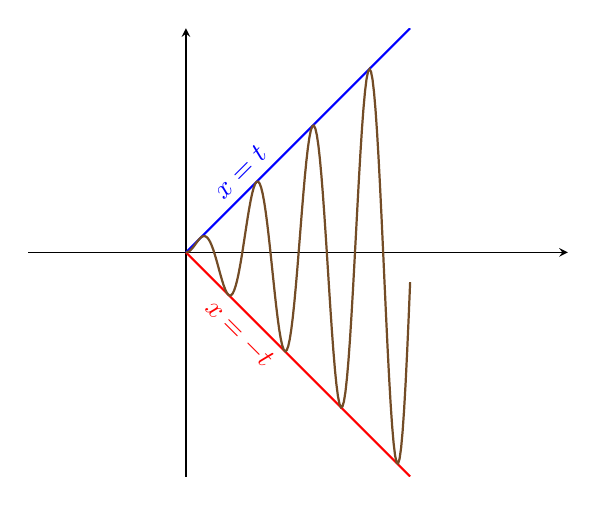
\begin{tikzpicture}
            \begin{axis}[domain=0:50,samples=150,
            %restrict y to domain=-5:5,
            xtick=\empty,ytick=\empty,
            %extra x ticks={0.8,1.4}, linea vertical
            %extra y ticks=3.333333,extra y tick labels={$\frac{10}{3}$}, linea horizontal
            %grid=both,
            axis lines=middle, axis equal
            ]
                \addplot+[no marks, thick] ({x},{x}) node[pos=0.3, above, sloped] {$x=t$};
                \addplot+[no marks, thick] ({x},{-x}) node[pos=0.3, below, sloped] {$x=-t$};
                \addplot+[no marks, thick] ({x},{x * sin(deg(x)/2)});
            \end{axis}
        \end{tikzpicture}
    \end{center}
    %%TODO: Añadir dibujo.
\end{eg}
\begin{obs}
    Como comentario, es más sencillo resolver las ecuaciones usando $e^{i \omega t},\ e^{-i \omega t}$ y luego separando la parte real e imaginaria.
\end{obs}
%%%%%%%%%%%%%%%%%%%%%%%%%%%%%%%%%%%%%%%%%%%%%%%%%%%%%%%%%%%%%%%% Clase del 20/02
\begin{eg}[Oscilador armónico amortiguado]
    Vamos a empezar considerando el muelle. En el oscilador armónico simple, teníamos $\mbf{x}'' = -\omega_0^2\mbf{x}$ (donde $-\omega_0^2 \mbf{x})$ era la fuerza de recuperación.\\
    Ahora, vamos a considerar el caso en el que exista el rozamiento. Sabemos que la fuerza de rozamiento es proporcional a la velocidad (para velocidades no muy grandes) en dirección contraria al movimiento. Es decir, tenemos: $(\mathcal{ED}) \equiv \mbf{x}'' = -\omega_0^2\mbf{x} - \mu \mbf{x}' \implies \mbf{x}'' + \mu \mbf{x}' + \omega_0^2\mbf{x} = 0$, que es una ecuación lineal homogénea. Por tanto su solución general es de la forma:
    $$
        x(t) = c_1 \mbf{x}_1 + c_2 \mbf{x}_2\ : \mbf{x}_1, \mbf{x}_2\text{ son linealmente independientes.}
    $$
    Para hallar $\mbf{x}_1$, $\mbf{x}_2$ resolvemos las raíces del polinomio característico: $\lambda^2 + \mu \lambda + \omega_0^2 = 0$. Distinguimos distintos casos:\\
    \begin{itemize}
        \item Caso $\sfrac{\mu}{2} > \omega_0$\\\\
        $$
            \lambda = -\frac{\mu}{2} \pm \sqrt{\left(\frac{mu}{2}^2\right) - \omega_0^2} \implies
            \begin{cases}
                \mbf{x}_1 = \mbf{x}_+ = e^{\lambda_+ t}\\
                \mbf{x}_2 = \mbf{x}_- = e^{\lambda_- t}
            \end{cases} \text{ con } \lambda_- < \lambda_+ < 0
        $$
        Y entonces, $\mbf{x}_-, \mbf{x}_+ \to 0$ cuando $t \to \infty$.
        \item Caso $\sfrac{\mu}{2} = \omega_0$\\\\
        Tenemos una raíz doble y las soluciones son:
        \begin{gather*}
            \mbf{x}_1 = e^{-\sfrac{\mu}{2} t}\\
            \mbf{x}_2 = t e^{-\sfrac{\mu}{2} t}
        \end{gather*}
        \item Caso $\sfrac{\mu}{2} < \omega_0$\\\\
        $$
            -\frac{\mu}{2} \pm i \sqrt{\omega_0^2 - \left(\frac{\mu}{2}\right)^2} = -\frac{\mu}{2} \pm i \omega_\mu
        $$
        y entonces, resolviendo la ecuación tenemos las soluciones:
        \begin{gather*}
            \mbf{x}_1 = e^{-\sfrac{\mu}{2} t} \cos(\omega_\mu t)\\
            \mbf{x}_2 = e^{-\sfrac{\mu}{2} t} \sin(\omega_\mu t)
        \end{gather*}
    \end{itemize}
\end{eg}
